\section{Ziel}
In diesem Versuch soll die Verdampfungswärme von Wasser bestimmt und die Dampfdruckkurve erstellt werden.
Außerdem wird die Temperaturabhängigkeit der Verdampfungswärme überprüft.
\section{Theorie}
\label{sec:Theorie}
Im Allgemeinen liegen Stoffe in einer der drei Phasen fest, flüssig oder gasförmig vor.
Ein Zustandsdiagramm kann die Phasen eines Stoffs darstellen. Dabei ist der Druck $\rho$ gegen die Temperatur $T$ aufgetragen. Innerhalb eines abgeschlossenen Bereichs 
hat das System zwei Freiheitsgrade. Das bedeutet, dass sich die Temperatur als auch der Druck ohne Phasenänderung ändern können. Wird jedoch eine Grenzlinie überschritten,
kommt es zu einer Phasenänderung. 
In diesem Versuch wird die Phasenänderung von flüssig auf gasförmig des Wassers untersucht. 
\begin{figure}
    \centering
    \caption{Zustandsdiagramm des Wassers.\cite{v203}}
    \label{fig:zus}
    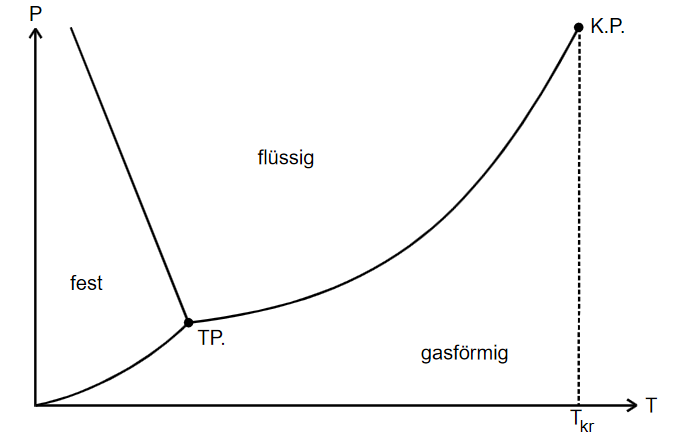
\includegraphics[width = 0.6 \textwidth]{pics/Phasendiagramm.png}
\end{figure}
Das Zustandsdiagramm von Wasser ist in Abbildung \ref{fig:zus} zu sehen. Die Dampfdruckkurve ist hierbei die Grenzlinie zwischen der festen und der gasförmigen Phase und befindet sich zwischen dem Tripelpunkt und dem kritischen Punkt.
An dem Tripelpunkt liegen alle drei Phasen vor, während am kritischen Punkt die gasförmige und flüssige Phase koexistieren. Der Verlauf der Kurve wird durch 
die Verdampfungswärme $L$ festgelegt, welche eine charakteristische Größe für jeden Stoff darstellt. Sie ist temperaturabhängig und verschwindet in der Nähe der Temperatur die
zum Kurvenpunkt K.P. gehört. Es existiert jedoch ein weiterer Temperaturbereich in dem $L$ nahezu konstant ist. Dort werden die Aufnahmen der Dampfdruckkurve und die Bestimmung
der Verdampfungswärme in diesem Versuch durchgeführt. 
\\
Die molare Verdampfungswärme $L$ gibt an wie viel Wärmeenergie nötig ist um ein Mol einer Flüssigkeit isotherm und isobar zu verdampfen. 
Die Verdampfung besteht darin, dass diejenigen Moleküle, die gemäß der Maxwellschen Geschwindigkeitsverteilung maximale kinetische Energie haben, die Flüssigkeitsoberfläche verlassen.
Um in die gasförmige Phase zu gelangen, müssen die Teilchen die molekulare Bindungskraft überwinden. Die dazu nötige Energie muss entweder von außen hinzugefügt werden oder dem Wasser entzogen werden, wodurch dieses abkühlt.
Auch im gasförmigen Zustand sind die Geschwindigkeiten Maxwell verteilt, weshalb der Prozess auch umgekehrt abläuft. Nach einiger Zeit stellt sich ein Gleichgewicht ein, wobei der dann herrschende Druck 
Sättigungsdampfdruck genannt wird. Da dieser Druck nicht vom Volumen des Gasraums abhängt, kann nicht mit der idealen Gasgleichung gerechnet werden.
Die Dampfdruckkurve kann mit Hilfe der Berechnung eines reversiblen Kreisprozess für ein Mol eines Stoffs hergeleitet werden. Dieser Kreisprozess ist in Abbildung \ref{fig:kreis} zu sehen.
\begin{figure}
    \centering
    \caption{Kreisprozess von Wasser im p-V-Diagramm.\cite{v203}}
    \label{fig:kreis}
    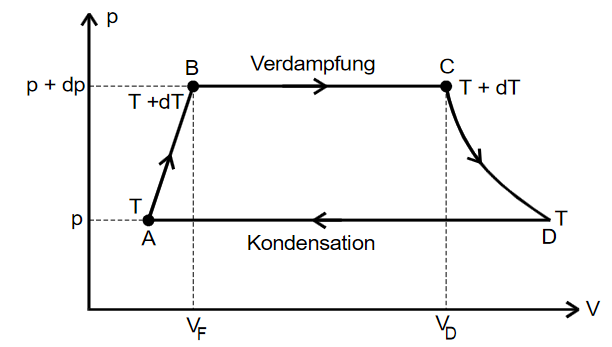
\includegraphics[width = 0.6 \textwidth]{pics/kreis.png}
\end{figure}
Dabei wird der Stoff zunächst isotherm und isobar verdampft und anschließend wieder kondensiert. Das Mol der Flüssigkeit wird aus dem Ausgangszustand A um eine Temperatur
$dT$ erhitzt, wobei sich auch der Druck um $dp$ erhöht. Nun wird die Flüssigkeit durch Zufuhr der Verdampfungswärme isotherm und isobar verdampft. Durch das Verdampfen
dehnt sich das Volumen von $V_F$ bis zu $V_D$ aus. Durch Wärmeentzug wird der Dampf auf die Temperatur $T$ abgekühlt, wobei sich der Druck auch auf den Ursprungswert $p$ reduziert.
Die Verdampfungswärme wird bei der isobar und isotherm erfolgenden Kondensation wieder freigesetzt. Bei der Aufsummierung aller Wärmeenergien der vier Vorgänge und
Gleichsetzung mit der insgesamt verrichteten Arbeit, folgt die Gleichung 
\begin{equation}
    (C_F-C_D) dT + dL = (V_D-V_F)dp \, .
\end{equation}
Dabei sind $C_F$ und $C_D$ die Molwärmen der Flüssigkeit beziehungsweise des Dampfes. 
$dL$ gibt den Unterschied der nötigen Verdampfungswärmen an, da diese bei höheren Temperaturen kleiner sind. Da ein reversibler Kreisprozess vorliegt, gilt nach dem zweitem Hauptsatz
der Thermodynamik 
\begin{equation}
    \sum_i \frac{Q_i}{T_i} = 0 \, ,
\end{equation}
woraus sich mit weiteren Vereinfachungen die Clausius-Clapeyronsche Gleichung
\begin{equation}
    (V_D-V_F)dp = \frac{L}{T}dT
    \label{eqn:claus}
\end{equation}
ergibt. Die Integration dieser Gleichung ist im allgemeinen Falle schwierig, da $V_D$, $V_F$ und $L$ komplizierte Funktionen der Temperatur sein können.
Allerdings können bei Temperaturen weit unter der kritischen Temperatur $T_{kr}$, die in Abbildung \ref{fig:kreis} eingeführt wurde und das obere Ende der Dampfdruckkurve beschreibt
folgende Näherungsannahmen genutzt werden. Diese lauten
\begin{itemize}
    \item $V_F$ ist gegenüber $V_D$ vernachlässigbar.
    \item $V_D$ lässt sich mir der idealen Gasgleichung
        \begin{equation}
            V_D(p,T) =R \frac{T}{p}
            \label{eqn:ideal}
        \end{equation}
        beschreiben.
    \item $L$ ist druck- und Temperaturunabhängig.
\end{itemize}
und daraus folgt durch Integration die Formel
\begin{equation}
    \ln p = - \frac{L}{R} \frac{1}{T} + \text{const}
    \label{eqn:log}
\end{equation}
oder
\begin{equation}
    p= p_0 \exp \left(- \frac{L}{R} \frac{1}{T}\right)
\end{equation}
mit der Konstanten $C= \ln p_0$.